\documentclass[11pt]{exam}
%%%%%%%%%%%%%%%%%%%%%%%%%%%%%%%%
\noprintanswers % pour enlever les réponses
%\printanswers

\unframedsolutions
\SolutionEmphasis{\itshape\small}
\renewcommand{\solutiontitle}{\noindent\textbf{A: }}
%%%%%%%%%%%%%%%%%%%%%%%%%%%%%%%%



%\usepackage[margin=0.73in]{geometry}
%\usepackage[top=1in, bottom=1in, left=1in, right=1in]{geometry}

%\usepackage{fullpage}


\usepackage{hyperref}
\usepackage{appendix}
\usepackage{enumerate}


\usepackage{times,graphicx,epsfig,amsmath,latexsym,amssymb,verbatim}%,revsymb}
\usepackage{algorithmicx, enumitem, algpseudocode, algorithm, caption}


%%%%%%%%%%%%%%%%%%%%%
% Handling comments and versions %%%
%%%%%%%%%%%%%%%%%%%%%
\newcommand{\extra}[1]{}

\renewcommand{\comment}[1]{\texttt{[#1]}}

\newcommand*{\ScProd}[2]{\ensuremath{\langle#1\!\mathbin{,}\!#2\rangle}} %Scalar Product


%%%%%%%%%%%%%%%%%%%%%%%%%%%
%% THEOREMS
%%%%%%%%%%%%%%%%%%%%%%%%%%%

\usepackage{amsmath,amssymb,amsfonts}
\usepackage{amsthm}

\newtheorem{theorem}{Theorem}[section]
\newtheorem{axiom}[theorem]{Axiom}
\newtheorem{conclusion}[theorem]{Conclusion}
\newtheorem{condition}[theorem]{Condition}
\newtheorem{conjecture}[theorem]{Conjecture}
\newtheorem{corollary}[theorem]{Corollary}
\newtheorem{criterion}[theorem]{Criterion}
\newtheorem{definition}[theorem]{Definition}
\newtheorem{lemma}[theorem]{Lemma}
\newtheorem{notation}[theorem]{Notation}
\newtheorem{proposition}[theorem]{Proposition}


\theoremstyle{definition}
\newtheorem{problem}{Problem}


\newcommand{\nc}{\newcommand}
\nc{\eps}{\varepsilon}
\nc{\RR}{{{\mathbb R}}}
\nc{\CC}{{{\mathbb C}}}
\nc{\FF}{{{\mathbb F}}}
\nc{\NN}{{{\mathbb N}}}
\nc{\ZZ}{{{\mathbb Z}}}
\nc{\PP}{{{\mathbb P}}}
\nc{\QQ}{{{\mathbb Q}}}
\nc{\UU}{{{\mathbb U}}}
\nc{\OO}{{{\mathbb O}}}
\nc{\EE}{{{\mathbb E}}}


\newcommand{\field}{\mathbb{K}}
\nc{\K}{K}
\newcommand{\M}{\mathcal{M}}
\newcommand{\val}{\operatorname{val}}
\newcommand{\bigO}{\mathcal{O}}
\DeclareMathOperator{\Span}{Span}
\newcommand{\vc}[1]{\mathbf{#1}}

\pretolerance=1000

%%%%%%%%%%%%%%%%%%%%%%%%%%%%%%%%
%%%%%%%%%%%%%%%%%%%%%%%%%%%%%%%%
%% DOCUMENT STARTS
%%%%%%%%%%%%%%%%%%%%%%%%%%%%%%%%
%%%%%%%%%%%%%%%%%%%%%%%%%%%%%%%%
\usepackage{tikz}
\usetikzlibrary{automata}
\DeclareMathOperator{\Vol}{Vol}

\begin{document}

{\noindent
   \textsc{ENS Lyon --  M1 -- Computer Algebra}
   \hfill {E.Kirshanova / A.Wallet // 2017--2018\\
  }
  \hrule
% Titre de la feuille
  \begin{center}
    {\Large\textbf{
   \textsc{Tutorial 8}
    } } 
  \end{center}
  \hrule \vspace{5mm}

\thispagestyle{empty}

\vspace{0.2cm}
\begin{center}
	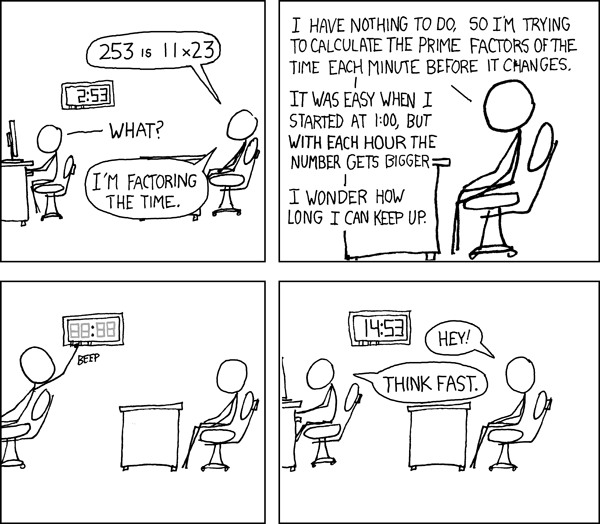
\includegraphics[scale=6]{factoring_the_time}
\end{center}


% \section{How to check if a number is a perfect power}
	
% 	Usually factorization algorithms assume that the input number $N$ we want to factor is not a perfect power. 
% 	Give an efficient algorithm that checks if $N $ is a perfect power, i.e., if $N = a^k$, and outputs the pair $(a,k)$ with the largest $k$.
% 		\begin{solution}
% 			Since $N = a^k$, $k  \le \log N$. For each integer $b$, we try binary search for $a$ from the set $\{ 2, \ldots, \lceil N^{1/b}\rceil\}$. Namely, for $\mathsf{mid} = (\frac{2+N^{1/b}}{2})^b$, check if  $\mathsf{mid}>N$, and if so, continue with the `left' sub-interval), or of $\mathsf{mid}<N$, in which case, continue to the right. Output $(\mathsf{mid}, b)$ in the case of the equality. 
			
% 			We have $< \log N$ possible choices for $b$. For each such choice, the number of $\mathsf{mid}'s$ is $\log(\lceil N^{1/b} \rceil) = \log \log N$. To get a $\mathsf{\mid}$, we raise to the power of $b$ which costs $\log b = \log \log N$ operations (in our case in $\RR$ with some precision). 
			
% 			The algorithm runs in time $O(\log N \cdot (\log \log N)^2)$.
			
% 			Guillaume suggested to take the $b$-th root of N for each choice of $b$. Likely the result won't be an integer (if it is, we're done). We search for a close-by integer. The above is the same where the search for the solution is performed in a binary-search manner.
% 		\end{solution}

\section{Pollard's $\rho$ for the factorization problem} 
In this exercise we develop a variant of the Pollard's $\rho$ method for factoring $N$. We assume that $p | N $ is the smallest (but still large for brute-force search) divisor of $N$.  Pollard's $\rho$ algorithm is an heuristic method: we assume that a certain deterministic sequence behaves like a truly random one.

The idea is to find two distinct $x, x' \in \ZZ_N$, s.t.\ $x - x' = 0 \mod p$. %(note that we do not know $p$, but $\gcd(x - x', n)$ reveals $p$).
The tuple $(x, x')$ defines a \emph{collision}. To find a collision efficiently, we define a random walk on $\ZZ_N$ as
\[
	f(x) = x^2 + a \mod N,  \quad a \in \ZZ_N
\] 
and consider a sequence $x_0, x_1, x_2, \ldots$ such that $x_i = f(x_{i-1})$ (we fix some initial $x_0$ to be a random element from $\ZZ_N$).
\begin{questions}
	\question Since $f$ takes values in a finite set, the sequence $(x_i)_i$ should eventually repeat itself. Show that you can expect to find a collision after $\mathcal{O}(\sqrt{p})$ steps. (\emph{Hint}: recall Birthday Paradox.) You should also be able to determine the constant in front of $\sqrt{p}$.
	\begin{solution}
		Draw the letter $\rho$ on the board having $x_1, \ldots, x_i$ as its tail and $x_{i+1}, \ldots$ as it's head (which is the cycle) to explain the origins of the algorithm's name.
		The complexity comes from a straightforward connection to the collision problem: let $X$ be a r.v.\ that gives a number of elements samples uniformly at random from a set of size $|S|$ before an element is sampled twice. Assume we have already selected $\ell$ distinct elements. The probability that the next element will differ from all the previous ones is $1-\ell/|S|$. Hence, $\Pr[X > \ell] = 1 \cdot (1-1/|S|)(1-2/|S|) \cdot \ldots \cdot (1-(\ell-1)/|S|)$. Using $1-x  < \exp(-x)$, we obtain $\Pr[X > \ell] \leq \exp(-(\ell-1)^2 / (2|S|)$. The expected value of $X$ is then (see, either Galbraith's book or Mitchenmacher\&Upfal)
		\begin{align*}
				\mathbb{E}[X] &= \sum_{i=1}^\infty X \Pr[X=i] = \sum_{i=1}^\infty i (\Pr[x>i-1] - \Pr[x>i]) = \sum_{i=0}^\infty (i+1-i) \Pr[X=i] = \\
									  &=\sum_{i=0}^\infty \Pr[X>\ell]  \leq 1 + \sum_{i=1}^\infty \exp(-(i-1)^2 / (2|S|) \approx 1 + \int_{x=0}^\infty \exp(x)^2 / (2|S|) dx \\
									  &= 1 + \sqrt{2 |S|} \int_{x=0}^{\infty} \exp(u)^2 du = 1+ \sqrt{(\pi/2)|S|}.
		\end{align*}
		In Pollard's algorithm, we assume that the sequence $x_i \bmod p$ is pseudorandom and $|S| = p$ and the constant is $\approx \sqrt{\pi/2}$. Most likely, the students know all the above from their probability course.
	
	\end{solution}
	\question Describe a Pollard's $\rho$ algorithm for factoring having the running time of order $\widetilde{\bigO} (\sqrt{p})$.
	\begin{solution}
		\begin{enumerate}
			\item Let $x_1$ be a random element from $\ZZ_{N}$ and $x_2 = f(x_1) \bmod N$. Let $d = 1$.
			\item Repeat the following steps until $ 1 < d < N $:
			\begin{itemize}
				\item $x_1 = f(x_1) \bmod N$
				\item $x_2 = f(f(x_2)) \bmod N$
				\item $d = \gcd(x_2 - x_1, N)$
			\end{itemize}
		\end{enumerate}
	Usually, one breaks the loop after a certain number of iterations and re-starts with a different choice of $x_1$ and/or $f$.
	\end{solution}
	\question Explain why the following choices for $f(x)$ are bad:
	\begin{itemize}
		\item $f(x) = ax+b \mod N$,  $a, b \in \ZZ_{N}$,
		\item $f(x) = x^2 \mod N$,
		\item $f(x) = x^2 - 2 \mod N$.
	\end{itemize}
	%Assume we know that $p = 1 \bmod m$ for a known $m>2$. Explain why the choice $f(x) = x^m+1$ is good.
	\begin{solution}
		\begin{itemize}
			\item if $a$ is invertible in $\ZZ_{N}$ (which is likely to be the case), the first choice for $f$ in a bijection, so the period will be of order $O(p)$ (the order of $a$ in $\ZZ_p$).
			\item the order of $\ZZ_p^*$ is $p-1$ (even) and in the sequence you will eventually get $x^{p-1} = 1 \bmod p$ and will get stuck with $1$'s as collisions, which are useless.
			\item If $x_1$ can be written as $x_1 = y + 1/y$, then $x_k = y^{2^k}+(1/y^{2^k})$. The resulting sequence is not pseudorandom. It probably results in long periods as well but I do not know how to argue about it.
		\end{itemize}
	
	\end{solution}
\end{questions}
	%\item Given $f(x) = x^2+1$ and $x_0 = 1$, factor $n = 899$.

\section{Modular roots and factoring}

The first goal of this exercise is to design an efficient algorithm to compute square roots in the group $\mathbb{Z}_N$. This problem is closely related to the one of factoring $N$. As a first step we study the Tonelli-Shanks algorithm to compute square roots modulo a prime $p$. In the next tutorial, we will extend it to the non-prime moduli.

The Euler criterion states that, for any odd prime $p$ and any $a\in \mathbb{Z}_p^\times$, we have
$$a^{(p-1)/2} \equiv \begin{cases} 1 \bmod p,\text{if~}a~\text{is a square modulo}~p\\
   -1 \bmod p,\text{if~}a~\text{is not a square modulo}~p.\end{cases}$$
  

\begin{questions}
  \question Assume $p\equiv 3 \bmod p$ and let $a$ be a square modulo $p$. Give an algorithm of binary complexity $O(\log^3 p)$ to compute a square root of $a$.
  \begin{solution}
    By Euler's criterion, $a^{(p-1)/2}\equiv 1 \bmod 4$, so that $a^{(p+1)/2} \equiv a\bmod p$. By assumption on $p$, we can write $(a^{(p+1)/4})^2 \equiv a\bmod p$ and thus $b=a^{(p+1)/4}$ is a square root of $a$ mod $p$. Fast exponentiation needs $\log p$ operations in $\mathbb{Z}_p^\times$, which gives the result.
  \end{solution}

  \question We now assume that $p\equiv 1 \bmod 4$, and write $p=2^vm+1$ with $v$ maximal and $m$ odd. Give a probabilistic algorithm that, given $p$, return $c \in \mathbb{Z}_p^\times$ which is not a square. What is its bit complexity? Show that $c^m$ generates the (unique) subgroup of order $2^v$ in $\mathbb Z_p^\times$.
  
  \begin{solution}
    We can write $p=2^hm+1$, with $m$ odd. The algorithm simply samples a random element in $\mathbb{Z}_p^\times$ and checks if it is a square. This can be done by using Euler's criterion for a $O(\log^3 p)$ bit complexity; with more efficient algorithms involving Legendre's symbol properties and quadratic reciprocity law, it can be done in $O(\log^2 p)$.

    The probability of success is $1/2$. Indeed, there are $(p-1)/2$ squares in $\mathbb Z_p^\times$. To show this, consider the group morphism $\mathbb Z_p^\times \rightarrow \mathbb Z_p^\times, x\mapsto x^2$. Its kernel contains the two elements $\pm 1$, and it cannot contain more because $\mathbb{Z}_p$ is a field, so the polynomial $x^2-1$ has at most $2$ roots. Since the image of this maps is exactly the set of squares in $\mathbb Z_p^\times$, we conclude by the first isomorphism theorem.

    By Euler's criterion, we have that $c^{(p-1)/2} \equiv -1 \bmod p$, so we obtain $(c^m)^{2^{v-1}} \equiv -1 \bmod p$. Hence the order of $c^m$ is a power of two, and it cannot be less than $v-1$ since it would contradict the fact that $c$ is not a square, and we can write $(c^m)^{2^{v-1}}=((c^m)^2)^2\dots)^2$). Thus $c^m$ generates the subgroup of order $2^v$. 
  \end{solution}

  \question Let $a$ be a square modulo $p$, and $c$ be the output of the previous algorithm. Show that $a^m$ belongs to the subgroup generated by $c^m$. Next, show how that computing a square root of $a$ modulo $p$ amounts to computing a discrete logarithm.

  \begin{solution}
    We have $a^{(p-1)/2}=a^{2^{v-1}m}\equiv 1 \bmod p$, implying $(a^m)^{2^v} \equiv 1 \bmod p$, which gives the first claim. Let $d=c^m$. There exist $x\in [2^{v}-1]$ such that $a^m = d^x \bmod p$. Using Euler's criterion again:
    $$ 1 = a^{(p-1)/2} = (a^m)^{(p-1)/2} = (d^x)^{(p-1)/2} = \big((c^m)^{(p-1)/2}\big)^x=(-1)^x.$$
    Therefore, $x$ is even. Using our oracle, we compute $x$, and using $a^{m+1} = d^xa \bmod p$ we find the square root as $a^{(m+1)/2}d^{-x/2}$.
  \end{solution}

  \question \textbf{Pohlig-Hellman's trick:} Let $G$ be a cyclic group of order $p^k$, where $k\geq 1$. For a given generator $g$ and $h=g^x$, show that we can compute $x$ amounts to computations of discrete logarithms in a group of order $p$. (Hint: write $x$ in base $p$.)

  \begin{solution}
    Let $x=x_0+x_1p+\dotsb+x_{k-1}p^{k-1}$ and observe that $h^{p^{k-1}} = g^{x_0p^{k-1}}=(g^{p^{k-1}})^{x_0}$. This says that we can find $x_0$ by computing an exponentiation of $h$ and solving a discrete logarithm problem in the group generated by $g^{p^{k-1}}$, which has order $p$. Once this is done, we further have $h^{p^{k-2}}=g^{x_0p^{k-2}+x_1p^{k-1}}$, where $x_0$ is known. Thus $(hg^{-x_0})^{p^{k-2}}=(g^{p^{k-1}})^{x_1}$, so that $x_1$ can be computed with a discret log algorithm in the same subgroup as before. Overall, $x$ is computed with $k$ discrete logs in a group of order $p$.
    
    Elena: I think it're reasonable to ask for the complexity of the algorithm as well to complete the description. 
    
  \end{solution}

  \question Deduce an algorithm to compute square roots modulo $p$.

  \begin{solution}
    First find $v$ and $m$ by shifting-adding. Find a non-square $c$ modulo $p$, and compute $d=c^m$. To compute the discrete log of $a^m$ in the subgroup generated by $d$, since we are in a group whose cardinality is a power of $2$, we can follow the next instructions:
    \begin{itemize}
    \item $b\gets a^m$; $t\gets 0$;
    \item for $i=0$ until $i=v-1$ do:
      \begin{itemize}
      \item if $(bd^t)^{2^{v-1-i}} \equiv -1 \bmod p$, $t\gets t+2^i$,  (done by shifting-adding again).
      \end{itemize}
    \item outputs $a^{(m+1)/2}d^{-t/2}$.
    \end{itemize}

  \end{solution}

  \question (\textbf{Bonus}) Prove Euler's criterion.
  \begin{solution}
    The little theorem of Fermat tells that $a^{p-1}\equiv 1 \bmod p$ for amm $a \in \mathbb{Z}_p^\times$. In other words, the elements of $\mathbb{Z}_p^\times$ are roots (modulo $p$) of the polynomial $X^{p-1}-1$. Since $\mathbb{Z}_p$ is a field, these are in fact exactly all the roots. Since $p-1$ is even we can write $X^{p-1}-1 = \big(X^{(p-1)/2}-1\big)\big(X^{(p-1)/2}+1\big)$. If $a\equiv b^2 \bmod p$, then it is a root of the left factor. We know that there are $\frac{p-1}{2}$ such elements, so squares are exactly the roots of the left factor. This means the non-squares are exactly the roots of the right factor, and the result follows.
    
  \end{solution}
  
\end{questions}
\section{Why not to choose primes close to $\sqrt{N}$ for RSA}
 
Assume one of the RSA primes is close to $\sqrt{N}$, more precisely,
\[ 
	|q - \sqrt{N}| < \sqrt[4]{N}.
\] 
Show how to factor $N$ in time $poly(\log N)$.
\emph{Hint}. You might want to use the following fact: for $N = pq$, $N =
\left( \frac{p+q}{2}\right)^2 - \left( \frac{p-q}{2}\right)^2.
$ Note that
the first summand is $\approx \sqrt{N}$, while the second one is small.

\begin{solution}
 We show that Fermat's factoring method finds a non-trivial divisor after a constant number of steps. Fermat's method consists in writing $N$ as $N=t^2 - s^2 $ where $t = \frac{q+p}{2}$ and $s = \frac{q-p}{2}$ and iterating over $t=\lfloor \sqrt{N} \rceil+1, \lfloor \sqrt{N} \rceil+2, \ldots$ until we get a perfect square value (this is true for the correct $t$ since $t^2 - N^2 = s^2$ for an integer $s$).
 
 In the following, we assume $q>p$. Assume further that the largest prime is close to $\sqrt{N}$, namely $q<\sqrt{N}+\sqrt[4]{N}$. Then $p= \frac{N}{q} = \frac{N(\sqrt{N}-\sqrt[4]{N})}{N-\sqrt{N}}>\sqrt{N}-\sqrt[4]{N}.$ This implies that $q-p < 2 (\sqrt[4]{N}+1)$. A case then we have $p$ close to $N$ is similar, namely: $p>\sqrt{N} - \sqrt[4]{N}$  implies that $q < \frac{N(\sqrt{N}+\sqrt[4]{N}+2)}{(\sqrt{N}-\sqrt[4]{N})(\sqrt{N}+\sqrt[4]{N}+1)} =  \frac{N(\sqrt{N}+\sqrt[4]{N}+2)}{N+\sqrt{N}-\sqrt[4]{N}} < \sqrt{N}+\sqrt[4]{N}+2$. Both cases lead to $q-p < 2 (\sqrt[4]{N}+1)$.
 
 Assume Fermat's test fails at $t = \lfloor \sqrt{N} \rceil+1$, that is it does not give a perfect square. Then, $s = \sqrt{t^2 - N} > \sqrt{\sqrt{N}+1}>\sqrt{2}\sqrt[4]{N}$. But this contradict the fact established above: $s  = \frac{q-p}{2} < \sqrt[4]{N}+1$. Hence, Fermat's test output the solution upon the first trail. Polynomial running time comes from the operations (squaring, taking the square root), and can be easily refined.
\end{solution}

\end{document}



%%% Local Variables:
%%% mode: latex
%%% TeX-master: t
%%% End:
